% !TeX root = ../main.tex

\section{Virtual Platform}

Virtual platform, conceptually equivalent to virtual prototype, is the mainstream approach to the design of systems-on-chip (SoC). It is a software framework that is typically written in SystemC and functionally represents hardware. Nonetheless, virtual platform is not the same as simulator. Typically, simulator is dedicated to modeling CPU, GPU, and any other type of processing units at a specific abstraction level. For example, Spike is an open source functional ISA simulator that simulates RISC-V processors at instruction level. Another example is Gem5, which is an open source cycle-accurate simulator that focuses more on microarchitecture details.
Virtual platform, on the other hand, has a larger scope. The following are its advantages:
\begin{itemize}
    \item \textbf{HW/SW Co-Design}: Virtual platform provides an integrated framework where hardware and software can be simulated and debugged simultaneously. It becomes straightforward to switch between hardware breakpoint and software breakpoint, which is not possible with real hardware. ~\cite{hw_sw_codesign}
    \item \textbf{Cost Reduction}: Without virtual platform, issues in hardware cannot be discovered until the actual hardware is available. In other words, another silicon tape out might be needed to fix hardware issues. And this costs millions or even billions of dollars.~\cite{virtual_platform} In contrast, virtual platform enables hardware issues to be discovered at earlier stage and hence saves a huge amount of costs. 
    \item \textbf{Early Software Development}: Fig~\ref{fig:virtual_platform_without} and ~\ref{fig:virtual_platform} highlight the differences . Without virtual platform, software development, such as firmware and driver, has to wait until real hardware is available.~\cite{early_sw_development} This results in either slower time-to-market or lower quality of software stack due to limited development time. Taking GPU for example, not only GPU performance but also GPU driver are keys to success in market. In other words, enabling early GPU driver development helps gaining market share.  
\end{itemize}

\begin{figure}
    \centering
    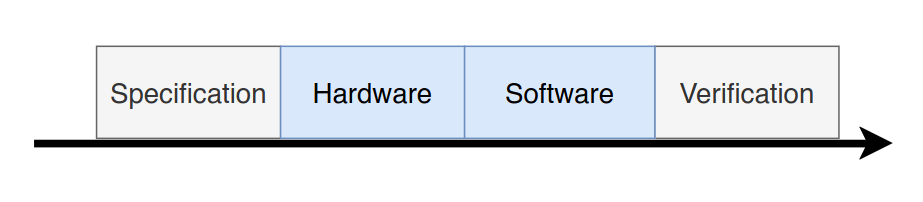
\includegraphics[width=.65\linewidth]{figures/Virtual_platform_without.png}
    \caption{SoC development without virtual platform}
    \label{fig:virtual_platform_without}
\end{figure}

\begin{figure}
    \centering
    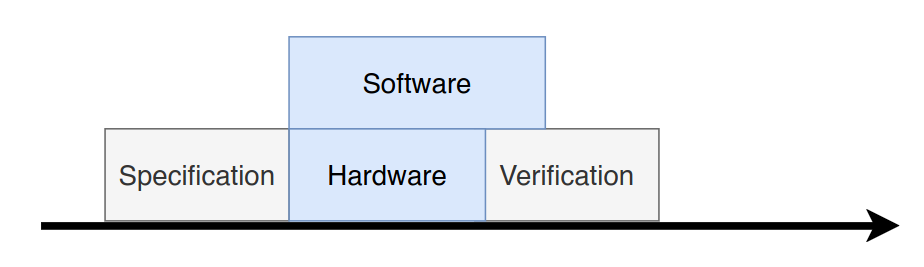
\includegraphics[width=.6\linewidth]{figures/Virtual_platform.png}
    \caption{SoC development with virtual platform}
    \label{fig:virtual_platform}
\end{figure}


\section{Performance Profiling Tools}
Performance profiling plays an important role in software development. In reality, there are always trade-offs between the amount of information available and profiling overhead. Generally speaking, there are two different profiling approaches, namely sampling and instrumentation:

\begin{itemize}
    \item \textbf{Sampling} is the most widely known and the less instrusive approach. Roughly speaking, it collects information about target software application periodically. The most representative sampling-based profiler is linux perf, also known as perf\_event. 
    \item \textbf{Instrumentation} 
\end{itemize}